%this file was autamatically generated by log_generator

%font size
\def\fontheight{14pt}

%class
\documentclass[a4paper, \fontheight]{article}

%packages
\usepackage[czech]{babel}           %language
\usepackage[a4paper, text={18cm,26cm}, left=1.5cm, top=2cm]{geometry}		%layout
\usepackage{times}					%font
\usepackage{multicol}
\usepackage{multirow}
\usepackage{graphicx}
\usepackage{float}
\usepackage{tabularx, booktabs}
\usepackage{tikz}
\usepackage{amssymb}

%encoding
\usepackage[IL2]{fontenc}           %font encoding
\usepackage[utf8]{inputenc}         %script encoding

\newcolumntype{s}{>{\hsize=0.2\hsize}X}
\newcolumntype{C}{>{\centering\arraybackslash}X}
\newcolumntype{S}{>{\hsize=0.2\hsize\centering\arraybackslash}X}

\begin{document}
	\pagenumbering{gobble}
	\begin{table}[H]
		\centering
		\ttfamily
			\begin{tabular*}{\textwidth}{l @{\extracolsep{\fill}} r}
			{\Large Operace: GHOST VERTEX} & \multirow[c]{3}{*}{
\includegraphics[scale=0.25]{./sources/CIA_logo.eps}} \\ [0.5em]
			{\Large Lokace: Základna CIA, Hoštejn} & \\ [0.5em]
			{\Large Jednotka: Alfa} & \\
\end{tabular*}
\end{table}

\vspace{4em}

\begin{table}[H]
\ttfamily
\catcode`\-=12
\begin{tabularx}{\textwidth}{C|C|l|s|s|s|s|s|s|S|}
\textbf{Datum} & \textbf{Čas} & \textbf{Záznam signálu} & \multicolumn{6}{l|}{\bfseries Zaznamenané lokace} & \textbf{\large \checkmark}\\ \toprule[0.4mm]
			&& \multirow[c]{3}{*}{\resizebox{0.33\columnwidth}{!}{
	\begin{tikzpicture}
		\draw [draw=none] (0,0) -- (0,5);	%%set height
		\draw [line width=2mm, black] plot [smooth, tension=0.7] coordinates { (0,3) (2,1) (4,1) (6,0) (8,0) (10,4) (12,3) (14,1) (16,5) (18,3) (20,2) (22,5) (24,4) (26,1) (28,5) (30,1) (32,5) (34,2) (36,4) (38,3) (40,1) (42,5) (44,0) (46,5) (48,2) (50,3) (52,2) (54,5) (56,3) (58,1) (60,1) (62,0) (64,0) (66,2) (68,0) (70,1) (72,4) (74,1) (76,0) (78,1) };
	\end{tikzpicture}}} &&&&&&& \\ \cline{4-9}
			&&&&&&&&& \\ \cline{4-9}
			&&&&&&&&& \\ \toprule[0.3mm]
			&& \multirow[c]{3}{*}{\resizebox{0.33\columnwidth}{!}{
	\begin{tikzpicture}
		\draw [draw=none] (0,0) -- (0,5);	%%set height
		\draw [line width=2mm, black] plot [smooth, tension=0.7] coordinates { (0,3) (2,5) (4,5) (6,5) (8,0) (10,5) (12,4) (14,0) (16,4) (18,1) (20,1) (22,0) (24,4) (26,4) (28,5) (30,5) (32,4) (34,0) (36,5) (38,2) (40,5) (42,1) (44,1) (46,5) (48,2) (50,0) (52,0) (54,0) (56,0) (58,0) (60,3) (62,4) (64,5) (66,0) (68,3) (70,0) (72,5) (74,0) (76,4) (78,4) };
	\end{tikzpicture}}} &&&&&&& \\ \cline{4-9}
			&&&&&&&&& \\ \cline{4-9}
			&&&&&&&&& \\ \toprule[0.3mm]
			&& \multirow[c]{3}{*}{\resizebox{0.33\columnwidth}{!}{
	\begin{tikzpicture}
		\draw [draw=none] (0,0) -- (0,5);	%%set height
		\draw [line width=2mm, black] plot [smooth, tension=0.7] coordinates { (0,0) (2,5) (4,0) (6,3) (8,5) (10,3) (12,4) (14,1) (16,0) (18,0) (20,1) (22,1) (24,4) (26,5) (28,5) (30,5) (32,1) (34,5) (36,5) (38,3) (40,3) (42,5) (44,3) (46,5) (48,1) (50,0) (52,3) (54,3) (56,3) (58,0) (60,3) (62,1) (64,3) (66,1) (68,4) (70,2) (72,2) (74,2) (76,1) (78,3) };
	\end{tikzpicture}}} &&&&&&& \\ \cline{4-9}
			&&&&&&&&& \\ \cline{4-9}
			&&&&&&&&& \\ \toprule[0.3mm]
			&& \multirow[c]{3}{*}{\resizebox{0.33\columnwidth}{!}{
	\begin{tikzpicture}
		\draw [draw=none] (0,0) -- (0,5);	%%set height
		\draw [line width=2mm, black] plot [smooth, tension=0.7] coordinates { (0,3) (2,1) (4,4) (6,2) (8,4) (10,1) (12,5) (14,5) (16,5) (18,0) (20,5) (22,2) (24,2) (26,0) (28,0) (30,3) (32,1) (34,3) (36,5) (38,5) (40,4) (42,1) (44,5) (46,5) (48,2) (50,5) (52,0) (54,4) (56,1) (58,0) (60,4) (62,4) (64,1) (66,2) (68,5) (70,4) (72,2) (74,4) (76,3) (78,1) };
	\end{tikzpicture}}} &&&&&&& \\ \cline{4-9}
			&&&&&&&&& \\ \cline{4-9}
			&&&&&&&&& \\ \toprule[0.3mm]
			&& \multirow[c]{3}{*}{\resizebox{0.33\columnwidth}{!}{
	\begin{tikzpicture}
		\draw [draw=none] (0,0) -- (0,5);	%%set height
		\draw [line width=2mm, black] plot [smooth, tension=0.7] coordinates { (0,2) (2,5) (4,3) (6,5) (8,2) (10,5) (12,5) (14,0) (16,5) (18,1) (20,3) (22,3) (24,4) (26,5) (28,3) (30,2) (32,3) (34,2) (36,4) (38,2) (40,0) (42,4) (44,5) (46,4) (48,5) (50,2) (52,5) (54,5) (56,1) (58,2) (60,1) (62,3) (64,5) (66,2) (68,1) (70,0) (72,2) (74,0) (76,0) (78,5) };
	\end{tikzpicture}}} &&&&&&& \\ \cline{4-9}
			&&&&&&&&& \\ \cline{4-9}
			&&&&&&&&& \\ \toprule[0.3mm]
		\end{tabularx}
	\end{table}

	\vspace{-1.5em}

    \noindent
	\begin{figure}[H]
	\centering
	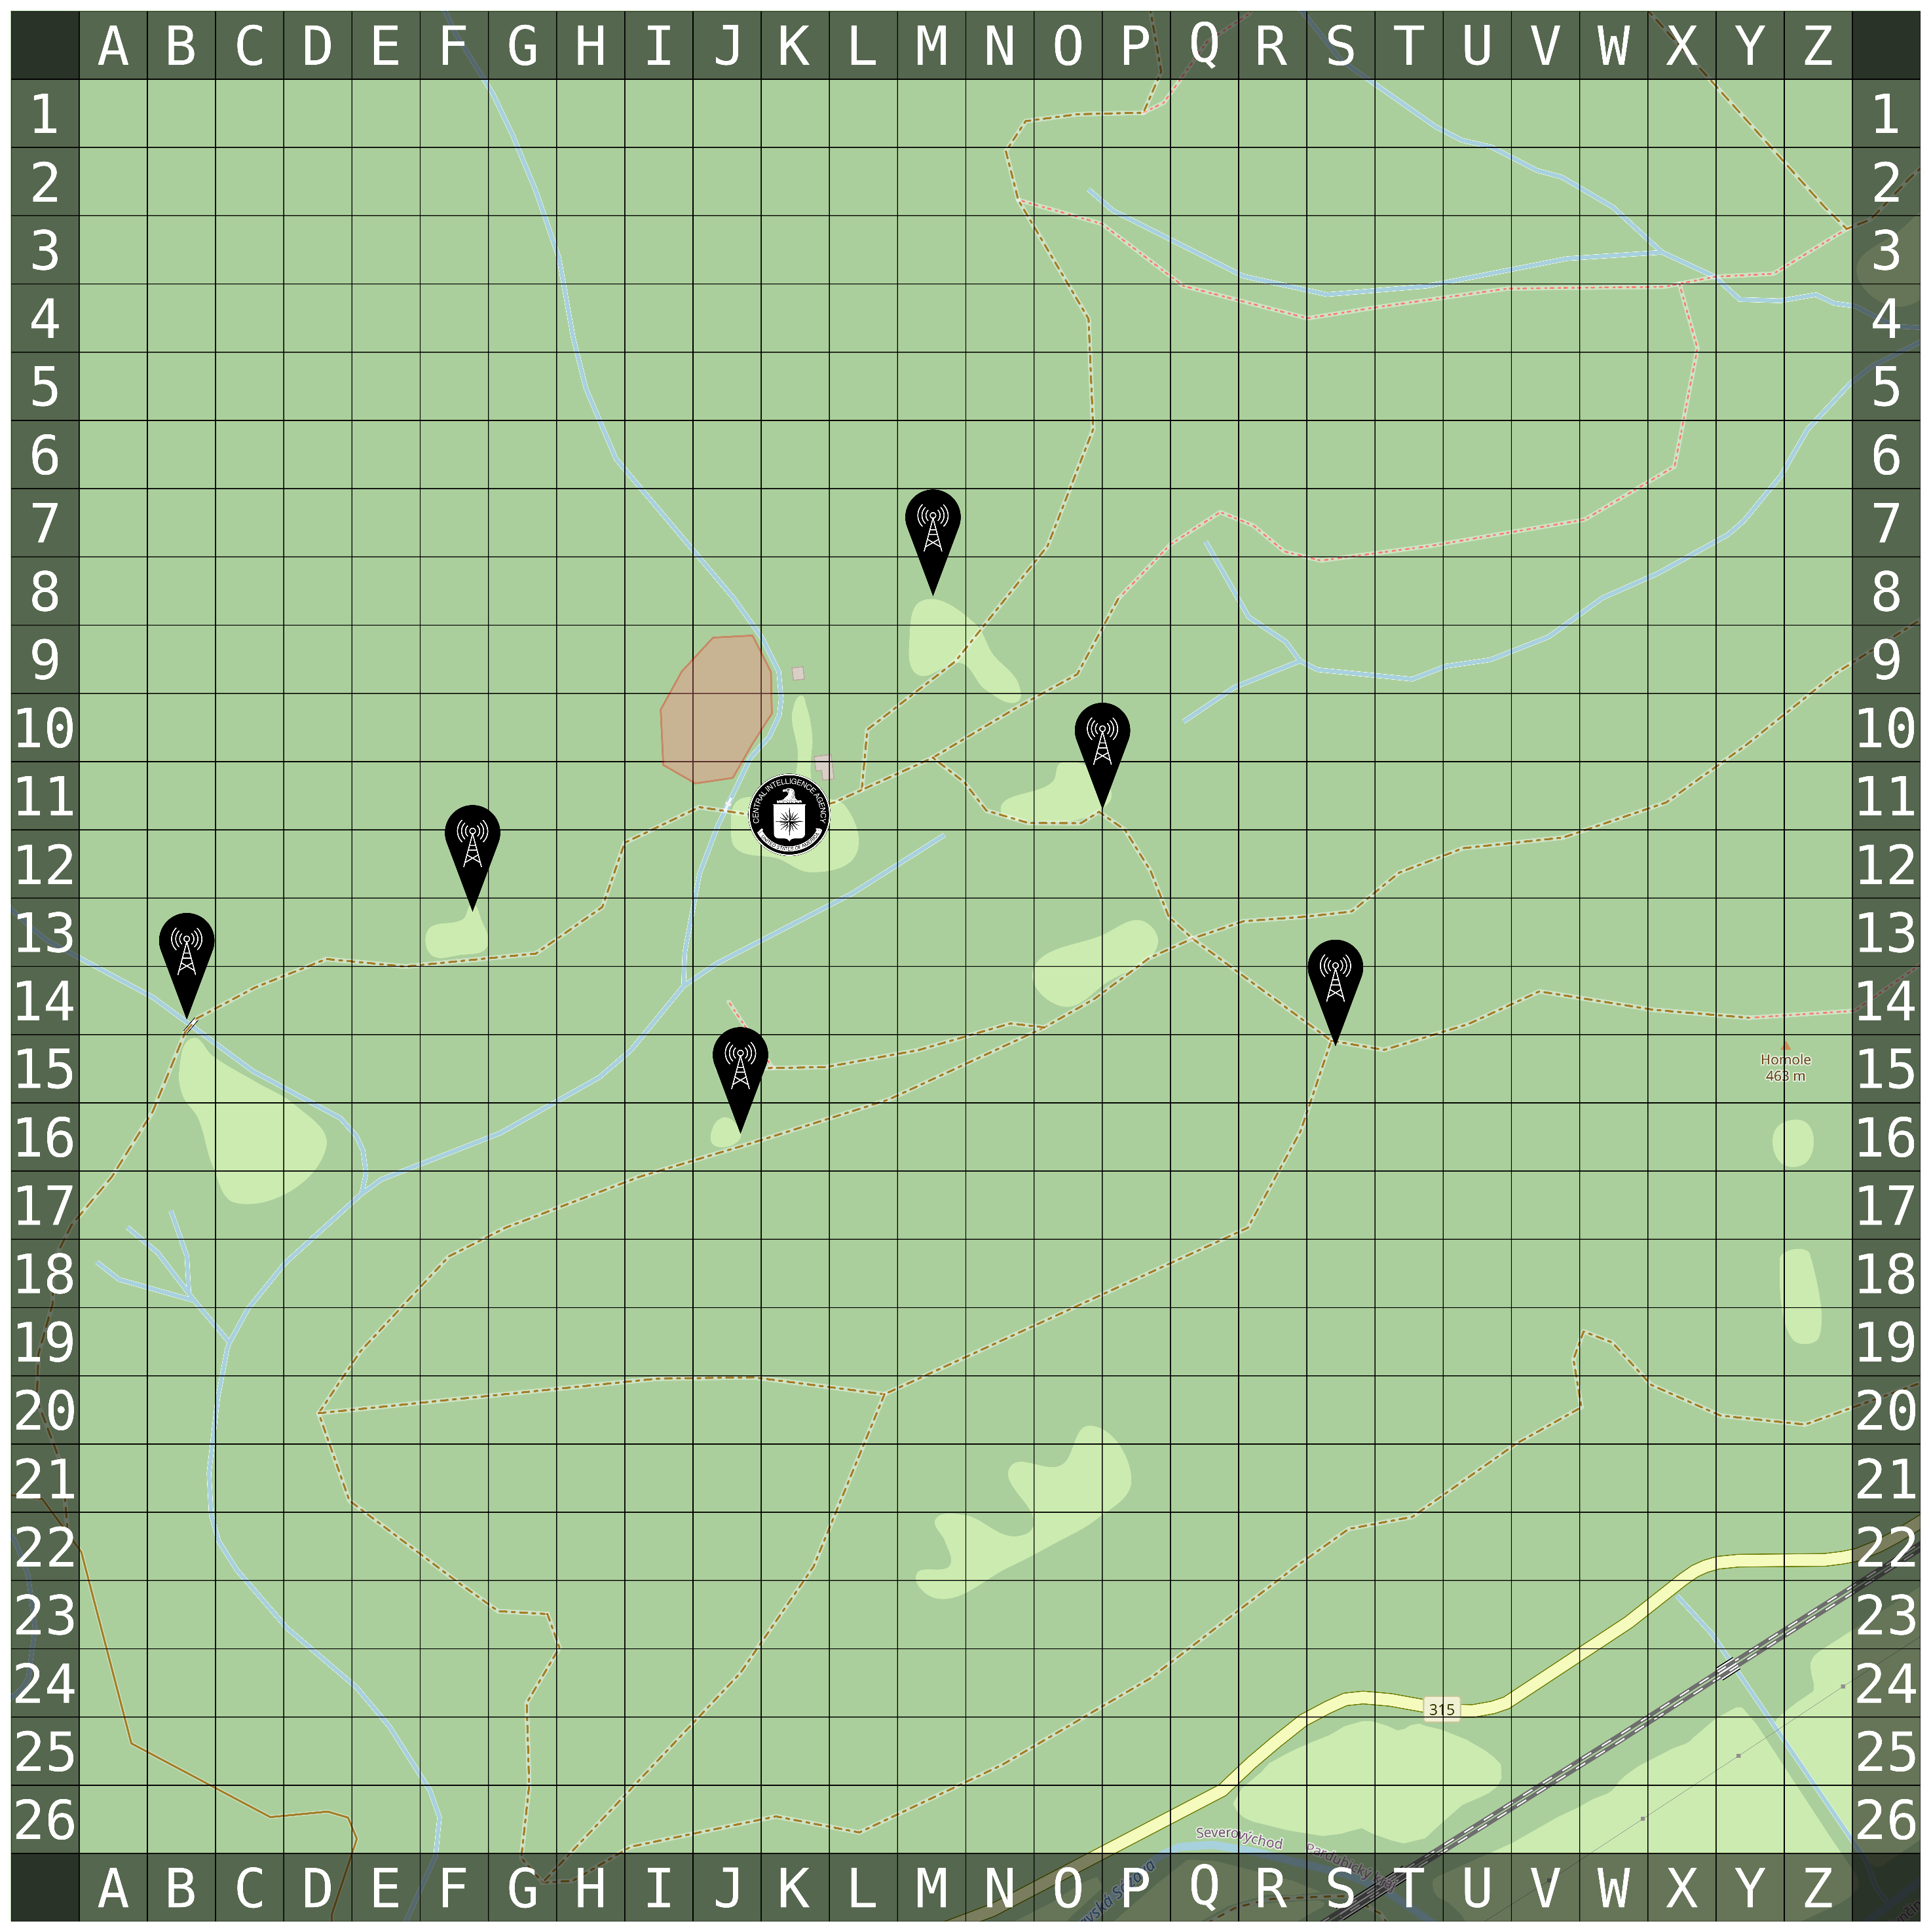
\includegraphics[scale=0.275]{./sources/map.eps}
	\end{figure}


\end{document}
